% template.tex, dated April 5 2013
% This is a template file for Annual Reviews 1 column Journals
%
% Compilation using ar-1col-S2O.cls' - version 1.0, Aptara Inc.
% (c) 2013 AR
%
% Steps to compile: latex latex latex
%
% For tracking purposes => this is v1.0 - Apr. 2013

\documentclass{ar-1col-S2O}
\usepackage{amssymb}
\usepackage{amsmath}
\usepackage[ruled,procnumbered]{algorithm2e}%
\usepackage[numbers]{natbib}
\usepackage[nameinlink]{cleveref}
\usepackage{listings}%
\usepackage{url}
\setcounter{secnumdepth}{4}

% Metadata Information
\jname{Xxxx. Xxx. Xxx. Xxx.}
\jvol{AA}
\jyear{YYYY}
\doi{10.1146/((please add article doi))}

% tikz libs
\usepackage{tikz} % fancy diagrams
\usetikzlibrary{positioning}
\usetikzlibrary{shapes,snakes}
\usetikzlibrary{arrows.meta}

% Change name of algorithm to "snippet"
\SetAlgorithmName{Snippet}{snippet}{list of snippets}
\makeatletter
\renewcommand{\algorithmautorefname}{Snippet}
\makeatother

%cref alias
\newcounter{snippet}
\makeatletter
% https://tex.stackexchange.com/a/212030/26355
\AtBeginEnvironment{snippet}{\let\c@algocf\c@snippet\crefalias{algocf}{snippet}}
\makeatother
\crefname{algorithm}{snip.}{snips.}
\Crefname{algorithm}{Snippet}{Snippets}


% Document starts
\begin{document}

% Page header
\markboth{Author et al.}{Short title}

% Title
\title{Machine Learning in Biology}


%Authors, affiliations address.
\author{Author B. Authorone,$^1$ Firstname C. Authortwo,$^2$ and D. Name Authorthree$^3$
\affil{$^1$Department/Institute, University, City, Country, Postal code; email: author@email.edu}
\affil{$^2$Department/Institute, University, City, Country, Postal code}
\affil{$^3$Department/Institute, University, City, Country, Postal code}}

%Abstract
\begin{abstract}
Abstract text, approximately 150 words. 
\end{abstract}

%Keywords, etc.
\begin{keywords}
keywords, separated by comma, no full stop, lowercase
\end{keywords}
\maketitle

%Table of Contents
\tableofcontents


% Heading 1
\section{INTRODUCTION}
Please begin the main text of your article here. 

%%% Fig of search terms
\begin{figure}[htb]
\centering
	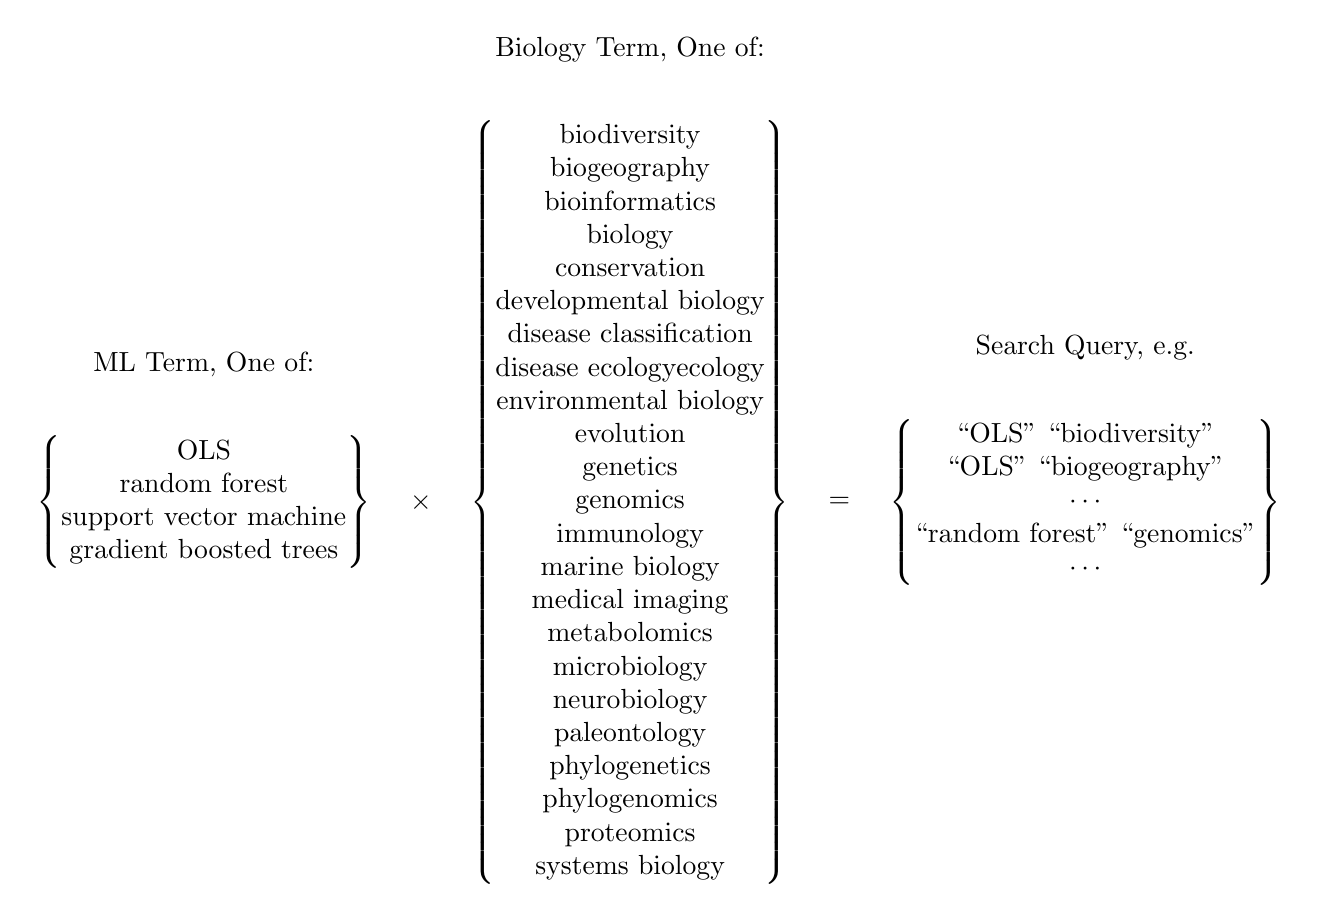
\begin{tikzpicture}[node distance=2.5cm,auto]
		\node[draw=none, anchor=north] (biot) {Biology Term, One of:};
        \node[below=0.5cm of biot] (bio) {$\left\{ \begin{matrix}
            \text{biodiversity} \\
            \text{biogeography} \\
            \text{bioinformatics} \\
            \text{biology} \\
            \text{conservation} \\
            \text{developmental biology} \\
            \text{disease classification} \\
            \text{disease ecology}
            \text{ecology} \\
            \text{environmental biology} \\
            \text{evolution} \\
            \text{genetics} \\
            \text{genomics} \\
            \text{immunology} \\
            \text{marine biology} \\
            \text{medical imaging} \\
            \text{metabolomics} \\
            \text{microbiology} \\
            \text{neurobiology} \\
            \text{paleontology} \\
            \text{phylogenetics} \\
            \text{phylogenomics} \\
            \text{proteomics} \\
            \text{systems biology} \\
        \end{matrix}\right\}$}; 
        \node[left=0.25cm of bio] (cross) {$\mathbf{\times}$};
        \node[left=0.25cm of cross] (ml) {$\left\{ \begin{matrix}
            \text{OLS} \\
            \text{random forest} \\
            \text{support vector machine} \\
            \text{gradient boosted trees} 
        \end{matrix}\right\}$}; 
		\node[above=0.5 of ml] (mlt) {ML Term, One of:}; 
        \node[right=0.25cm of bio] (equals) {$\mathbf{=}$};
        \node[right=0.25cm of equals] (query) {$\left\{ \begin{matrix}
            \text{``OLS'' ``biodiversity''} \\
            \text{``OLS'' ``biogeography''} \\
            \cdots \\
            \text{``random forest'' ``genomics''} \\
            \cdots \\
        \end{matrix}\right\}$}; 
		\node[above=0.5 of query] (queryt) {Search Query, e.g.}; 
		%\node[draw, circle, minimum size=1.5cm, left=2cm of dummy] (x) {$P(x)$}; 
		%\node[draw, circle, minimum size=1.5cm, right=2cm of dummy] (x2) {$P(x')$}; 
		%\node[draw=none, below=0.5cm of dummy] (pmf2) {$A(x,x')q(x,x')$}; 
%
		%\draw[-{Latex[length=3mm]}] (x.north east) -- (x2.north west);
		%\draw[{Latex[length=3mm]}-] (x.south east) -- (x2.south west);

		%\node[draw=none, below=2cm of dummy] (db) {Detailed Balance: $A(x',x)q(x',x)P(x) = A(x,x')q(x,x')P(x')$}; 
	\end{tikzpicture}
    \caption{Construction of search queries by selecting one machine learning term and one biology term.}
    \label{fig:search}
\end{figure}



\subsection{Ordinary Least Squares}
Ordinary Least Squares (OLS) is a
  statistical method utilized to estimate the parameters of a linear
  regression model. This technique focuses on minimizing the sum of the
  squares of the residuals---the differences between observed values in
  the dataset and the values predicted by the model. This approach
  ensures that the model fits as closely as possible to the data,
  providing a reliable basis for predictions and analysis.

In the formulation of a linear regression model, the relationship
between the dependent variable, denoted as \(y_{i}\) ,
and a set of independent variables, represented by the matrix
\(x_{i}\) , is typically expressed through the
equation
\(y_{i}\mathit{= \ }\mathit{\alpha\  + \ }\mathit{\beta}x_{i}\)
, Here \(y_{i}\) response variable that we are trying
to predict based on \(x_{i}\) , which comprises the
input features. The coefficients \(\mathit{\beta}\) represent the
parameters of the regression, indicating the influence of each input
feature on the dependent variable. The term \(\mathit{\alpha}\) is the
intercept, capturing the baseline value of \(y_{i}\)
when all \(x_{i}\) values are zero.

$$
\beta = \frac{\sum_{i = 1}^{n}{(x_{i}-\overline{x})(y_{i}-\overline{y})}}{\sum_{i = 1}^{n}{(x_{i}-\overline{x})}^{2}}
$$

$$
\alpha  = \overline{y}\  - \beta\overline{x}
$$

By solving the equation above finally we will get the model equation
like this:

$$
y_{i}= \alpha  + \beta x_{i}
$$

OLS is a basic and widely used method; however, it relies on various
assumptions that are violated in many datasets/research questions, e.g.
normally distributed errors and independent data points. For instance,
in a dataset with phylogenetic relationships between observations, OLS
may not reveal a relationship between variables within clades but not
across them, or show a relationship between variables across clades that
does not exist once phylogeny is accounted for~- in this case, PGLS
incoporating a variance-covariance matrix may be used (Symonds \&
Bomberg 2018). It is therefore often compared with newer ML techniques
in more recent papers.

\subsubsection{Implementation}

\begin{algorithm}
    \caption{Python OLS example}\label{alg:ols_py}
\begin{lstlisting}[language=R]
from sklearn.linear_model import LinearRegression
model = LinearRegression()
model.fit(Xtrain, Ytrain)
pred = model.predict(Xtest)
\end{lstlisting}
\end{algorithm}

\begin{algorithm}
    \caption{R OLS example}\label{alg:ols_r}
\begin{lstlisting}[language=R]
library(stats)
#fit the model with training data
ols.model <- lm(formula = outcome ~ predictor, data = training)
preds <- predict(ols.model, newdata=testing)
\end{lstlisting}
\end{algorithm}


References

Dalgaard, Peter. \emph{Introductory Statistics with R}. Statistics and
Computing. New York, NY: Springer New York, 2008.
https://doi.org/10.1007/978-0-387-79054-1.

Symonds, Matthew R. E., and Simon P. Blomberg. ``A Primer on
Phylogenetic Generalised Least Squares.'' In \emph{Modern Phylogenetic
Comparative Methods and Their Application in Evolutionary Biology},
edited by László Zsolt Garamszegi, 105--30. Berlin, Heidelberg: Springer
Berlin Heidelberg, 2014. https://doi.org/10.1007/978-3-662-43550-2\_5.

James, G., Witten, D., Hastie, T., Tibshirani, R. \& Taylor, J., 2023.
An introduction to statistical learning with applications in Python.
Springer.

Support Vector machines (SVMs) are a set of supervised learning methods
widely used for applications such as image classification, text
classification, and bioinformatics routines. SVMs are often used for
classification but can also be adapted for regression tasks. Before the
1980s almost all learning methods learned linear decision surfaces, and
the amount of samples in statistical studies tended to be infinite.
However, the size of real life the datasets is usually limited and the
relationships between the features is almost never linear. In 1995,
Vladimir N. Vapnik developed a novel approach and showed that SVMs work
well with nonlinear and high-dimensional datasets at pattern recognition
routines (Vapnik, 1995). Based on the concept of similarity, SVMs uses
kernel functions to transform the data to a higher dimensionality,
enabling linear separation by finding optimal hyperplanes that form the
best decision boundary between classes and Support vectors or the data
points that lie closest to the decision surface (or hyperplane) to
maximize the margins between the classes. SVMs are flexible in defining
similarity measures and often generalizes well to new data. With the
advantage of global optimization and strong adaptability it has wide
applications in areas like protein classification and face recognition.

SVMs are primarily focused with determining the hyperplane the optimally
divides data into particular classes based on the maximum margin
(Vapnik, 1995; Cortes and Vapnik, 1995). The hyperplane on itself, is
specifically defined such that on the minimum distance between data
points in different groups (i.e. also known as support vectors) is
maximized. In the case of pairwise data,

$\left( x_{i},\ y_{i} \right)$, where
$\left( x_{i}\  \in \ {\mathbb{R}}^{n} \right)$ are the
feature vectors and
$\left( y_{i}\  \in \ \left\{ 1,\  - 1 \right\} \right)$ are the class
labels, SVMs are focused on solving the following optimization
problem:

\[\left\lbrack \min_{w,\ b}\ \frac{1}{2}\ \left\| w_{}^{2}\  + \ C\ \sum_{i = 1}^{m}\ \xi_{i} \right\rbrack \right.\ \]


\(\left( y_{i}\ \left( w\  \cdot \ x_{i}\  + \ b \right)\  \geq \ 1\  - \ \xi_{i} \right)\)
 \((i)\)
\(\backslash\left( \xi_{i}\  \geq \ 0\backslash \right)\) are slack
variables that allow misclassification of either challenging or noisy
points. Similarly, \(\backslash(C\backslash)\ \) is a
regularization parameter that enables the control of the trade-off
associated with achieving a high margin while reducing training error.

Kernels are the source of the intrinsic flexibility and importance
in SVMs (Schölkopf and Smola, 2002). Kernels allow for operations in the
input space to be equivalent to operations in a higher dimensional
feature space (Hsu et al. 2003). Importantly, these operations occur
implicitly without the need of computing coordinates in the new
particular novel space (Noble, 2006). For instance, assume that although
elevation distinguishes between two populations, this feature was not
included in the analyzed dataset. Under SVMs, the use of a particular
kernel the collected dataset (e.g. latitude and temperature) might
result in the indirect inclusion of elevation as the result of the
expanded multivariate space.

A kernel function, $k\left( x_{i},x_{j} \right)$, is the dot product of two vectors of higher dimensional space.  Commonly used kernels functions polynomial kernel $k\left( x_{i},x_{j} \right)\  = \left( \gamma x_{i} \cdot x_{j}\  + r \right)^{d}$,
radial basis function (RBF) kernel,
$k\left( x_{i},x_{j} \right) = \exp\left( - \gamma\left\| x_{i} - x_{j}\right \|^{2} \right)$
,
and sigmoid kernel
$k\left( x_{i},x_{j} \right) = \tanh\left( \gamma x_{i} \cdot x_{j} + r \right)$,
where
 $\gamma, r$,  and $d$
are parameters that can be
adjusted based on the dataset.

\subsubsection{Usage in Biological research (Tanisha \& Cristian)}


\emph{Case study: MRI brain classification using support vector
machine:} In this paper, Support Vector Machines (SVM) are used for
classifying MRI brain images into normal and abnormal categories. The
methodology involves feature extraction through wavelet transformation,
specifically using Daubechies-4 wavelets to handle the data efficiently.
The extracted features then serve as input for the SVM classifier. The
SVM model operates by mapping input data into a higher-dimensional space
using an RBF kernel and then finding the optimal hyperplane that
separates the classes with the maximum margin. This approach is geared
towards improving the accuracy of classifying MRI scans, addressing the
challenge of distinguishing between normal and pathological features
effectively. The system is tested on a data set, and the results
highlight its potential, though challenges like computational complexity
and data precision limitations are noted.

\subsubsection{Implementation details}

SVMs are implemented in a range of libraries both in Python and R. In
Python, the primary library for implementing SVMs is Scikit-learn. This
versatile library implements functions to fit an analyze SVMs including
SVC (Support Vector Classification), SVR (Support Vector Regression),
and LinearSVC, an implementation that supports linear and non-linear
SVMs.

\begin{algorithm}
	\caption{Python SVM example using \texttt{sklearn}}\label{alg:svm_py}
\begin{lstlisting}[language=Python]
from sklearn import svm
# For classification
clf = svm.SVC(kernel='linear')
clf.fit(X_train, y_train)
predictions = clf.predict(X_test)
# For regression
reg = svm.SVR(kernel='linear')
reg.fit(X_train, y_train)
predictions = reg.predict(X_test)
\end{lstlisting}
\end{algorithm}


Within Python, the BioPython toolkit is closely integrated
SVM-related implementations. In R, the e1071 package, a wrapper of
the LIBSVM C++ library, is standard for implementing SVMs:

\begin{algorithm}
\caption{R SVM example using \texttt{e1071}}\label{alg:svm_r}
\begin{lstlisting}[language=Python]
library(e1071)
# For classification
model <- svm(formula = class ~ ., data =
    training_data, type =
'C-classification', kernel =
'linear')
predictions <- predict(model, newdata = test_data)
# For regression
model <- svm(y ~ ., data = training_data,
type = 'eps-regression', kernel =
'linear')
predictions <- predict(model, newdata = test\_data)
\end{lstlisting}
\end{algorithm}

Alternatively, excellent implementations of SVMs can be found in the
\texttt{tidymodels} R package, which offers a streamlined and modern framework
for modeling within R. The package includes functions such as
\texttt{svm\_rbf()} and \texttt{svm\_linear()} that facilitate the application of SVMs
with different kernel types in both regression and classification
tasks.

When fitting SVMs using \texttt{tidymodels}, practitioners typically focus
on three critical parameters to optimize their models. First, the choice
of the kernel type is central to this task as it determines the
transformation space of the input data. Common kernels include linear,
radial basis function (RBF), and polynomial. Each of this kernels is
particularly suited for different characteristics of the data. For
instance, the linear kernel is preferred for data that are linearly
separable in the input space. The RBF kernel can handle more complex,
nonlinear relationships. Second, tuning the regularization parameters,
particularly the penalty parameter, $C$, and
the kernel-specific parameter, $\gamma$.
These two parameters are essential for preventing overfitting and
ensuring the model generalizes well to new data. The parameter
$C$ controls the trade-off between achieving
a low error on the training data and minimizing the model complexity for
better generalization. The
$\gamma$ parameter defines how far the
influence of a single training example reaches. Specifically, low values
of $\gamma$ indicate ``far'' and high values
meaning ``close''. Third, defining the optimal value for the margin (i.e.
the decision boundary) is crucial. A larger margin can increase the
generalizability of the classifier. However, if the margin is set too
wide, it might lead to misclassification of the training data,
especially if the data are noisy or not well-separated.

There are considerations on pre-processing and interpretability of
the models. First, pre-processing of datasets analyzed using SVMs
generally involves several crucial steps. Normalization, for instance,
is critical as SVMs are not scale invariant, and thus features need to
be scaled typically to have zero mean and unit variance to ensure the
model does not bias toward attributes with higher magnitude values.
Imputation is employed to handle missing data values, which is common in
biological datasets. Balancing is particularly important in
classification tasks where class distributions are uneven, as unbalanced
datasets can lead to biased models that may overpredict the majority
class. Second, relative to simpler models, the interpretabilityof SVMs
is generally challenging. Overall, the main focus is generally directed
towards understanding the estimated weights. However, since the use of
kernels often yield to the exploration of novel multivariate spaces,
understanding the structure of results in SVMs in the context of the
biological question is not always straightforward. We will, however,
review two case of study in which SVMs were successfully used to
answering questions in the field.

HPC You et al. 2015



You, Y., Fu, H., Song, S. L., Randles, A., Kerbyson, D., Marquez, A.,
... \& Hoisie, A. (2015). Scaling support vector machines on modern HPC
platforms. \emph{Journal of Parallel and Distributed Computing},
\emph{76}, 16-31.





Cortes, C., \& Vapnik, V. (1995). Support-vector networks. Machine
learning, 20(3), 273-297.

Schölkopf, B., \& Smola, A. J. (2002). Learning with Kernels:
Support Vector Machines, Regularization, Optimization, and Beyond.

Hsu, C. W., Chang, C. C., \& Lin, C. J. (2003). A practical guide to
support vector classification.

Noble, W. S. (2006). What is a support vector machine? Nature
Biotechnology, 24(12), 1565-1567.

Vapnik, V., Golowich, S.E. and Smola, A.J. (1997) Support Vector
Method for Function Approximation, Regression Estimation and Signal. In:
Mozer, M.C., Jordan, M. and Petsche, T., Eds., Advances in Neural
Information Processing Systems 9, MIT Press, Cambridge, 281-287.
(\url{https://proceedings.neurips.cc/paper_files/paper/1996/file/4f284803bd0966cc24fa8683a34afc6e-Paper.pdf}{Support
Vector Method for Function Approximation, Regression Estimation, and
Signal Processing})

Othman, Mohd Fauzi Bin, Noramalina Bt Abdullah, and Nurul Fazrena Bt
Kamal. "MRI brain classification using support vector machine." 2011
fourth international conference on modeling, simulation and applied
optimization. IEEE,
2011.(\url{https://ieeexplore.ieee.org/abstract/document/5775605/})


\subsection{Random Forest}

\begin{itemize}
\item
  \emph{\textbf{Introduction to Random Forest}}: Random forest is a
  machine learning technique that has gained widespread popularity for
  their versatility and effectiveness in various prediction tasks
  (Breiman 2001, Epifanio 2017). This approach, which comprises an
  ensemble of decision trees and seamlessly integrates feature selection
  and interactions into the learning process, is highly favored by
  researchers and practitioners alike (Breiman 2001, Brieuc et al. 2018,
  Fabris et al 2018). Random forests have been successfully applied
  across diverse domains such as posttranslational modification site
  prediction, fold recognition, protein-protein interaction site
  prediction, enzyme function classification, and interaction or
  association between molecular markers and phenotype (Fraimout et al.
  2017, Brieuc et al. 2018, Fabris et al 2018).
\item
  \textbf{Technical overview of random forest:}
\end{itemize}

\begin{quote}
\textbf{Description of Random Forest:} Random Forest is a versatile and
powerful machine learning algorithm used for both classification and
regression tasks (Breiman 2001). It belongs to the ensemble learning
family, which combines multiple individual models to improve overall
predictive performance. The "forest" in Random Forest is composed of a
collection of decision trees.
\end{quote}

\includegraphics[width=3.02722in,height=1.71542in]{figs/rf.png}

\begin{enumerate}
\def\labelenumi{\alph{enumi}.}
\item
  \textbf{Decision Trees:} Each tree in the forest is a decision tree,
  which is a flowchart-like structure where an internal node represents
  a feature or attribute, the branch represents a decision rule, and
  each leaf node represents the outcome. Decision trees are simple yet
  effective models for classification and regression (Hastie et al.
  2009).
\end{enumerate}

\includegraphics[width=2.22832in,height=1.69421in]{figs/tree.png}

\begin{enumerate}
\def\labelenumi{\alph{enumi}.}
\setcounter{enumi}{1}
\item
  \textbf{Randomness:} Random Forest introduces randomness in two key
  ways (Breiman 2001):

  \begin{itemize}
  \item
    Random Sampling: During the training phase, instead of using the
    entire dataset to build each tree, Random Forest randomly selects a
    subset of the data (with replacement), known as bootstrap samples.
  \item
    Random Feature Selection: At each node of the decision tree, instead
    of considering all features to determine the best split, Random
    Forest randomly selects a subset of features. This introduces
    diversity among the trees and prevents overfitting.
  \end{itemize}
\item
  \textbf{Voting or Averaging:} For classification tasks, Random Forest
  combines the predictions of all the individual trees by majority
  voting, i.e., the class that receives the most votes. For regression
  tasks, it averages the predictions made by all the trees to obtain the
  final prediction (Breiman L. 2001).
\end{enumerate}

\begin{itemize}
\item
  \textbf{Training Techniques and Optimization Algorithms:}

  \begin{enumerate}
  \item
    Bootstrap Aggregating (Bagging): Random Forest employs a technique
    called bagging, which involves training each decision tree on a
    random subset of the training data with replacement. This helps in
    reducing overfitting by introducing diversity among the trees.
  \item
    Decision Tree Construction: Each decision tree in the Random Forest
    is constructed using a subset of features selected randomly at each
    node. This randomness ensures that the trees are less correlated
    with each other, leading to a more robust model.
  \item
    Number of Trees (n\_estimators): One of the hyperparameters of
    Random Forest is the number of trees in the forest. Typically,
    increasing the number of trees improves performance, but it also
    increases computational cost. Finding the optimal number of trees
    often involves cross-validation techniques.
  \item
    Feature Importance: Random Forest provides a measure of feature
    importance, which indicates the contribution of each feature in
    predicting the target variable. This information can be useful for
    feature selection and understanding the underlying data.
  \item
    Parallelization: Training each decision tree in Random Forest is
    independent of the others, making it highly parallelizable. Many
    implementations of Random Forest leverage parallel computing to
    speed up the training process, especially when dealing with large
    datasets.
  \item
    Hyperparameter Tuning: Random Forest has several hyperparameters
    such as the number of features to consider at each split, maximum
    depth of the trees, minimum samples per leaf, etc. Grid search or
    randomized search techniques can be used to find the optimal
    combination of hyperparameters (Hastie et al. 2009).
  \end{enumerate}
\end{itemize}

\begin{itemize}
\item
  \textbf{Usage in biological research}.
\end{itemize}

\begin{quote}
\textbf{Case 1:} A practical introduction to random forest for genetic
association studies in ecology and evolution.. In case 1, they used R.
They were looking at the association between molecular markers and
phenotype.

\textbf{Case 2:} a new approach for interpretation random forest models
and its application to the biology of aging. In case 2, they used Linux
Mint. They were trying to predict the expression of genes in brain
aging.
\end{quote}

\begin{itemize}
\item
  \textbf{Implementation details}:
\end{itemize}

\begin{quote}
\textbf{Case 1}: In this study, they explore the use of Random Forest
(RF) to discern loci underlying both discrete and quantitative traits,
particularly when studying wild or nonmodel organisms. RF is becoming
increasingly used in ecological and population genetics because, unlike
traditional methods, it can efficiently analyze thousands of loci
simultaneously and account for nonadditive interactions. They described
to prepare data for RF, including initial data exploration and the
identification of important covariates and possible confounding factors.
They next provide guidance on the initiation of RF and the optimization
of the algorithm parameters for classification and regression. Last,
they summarize methods for interpreting the results of RF and
identifying trait-associated, or predictor, loci (Fabris et al 2018).

\textbf{Case 2}: In this study, the authors were looking at how we can
use RF to predict when a gene is being over expressed, under expressed
or has no change in the brain when aging. The author use Linux Mint. To
look for the association of gene expression and aging, the author
created a dataset with different type of gene that are improved in
aging. Following that, the author evaluated the precise accuracy using
the Area Under the Receiver Operating Characteristic curve (AUROC),
computed via 10-fold cross-validation. AUROC values indicate the model's
performance, with 1.0 representing perfect classification. 10-fold
cross-validation is utilized for AUROC calculation, with the mean value
obtained over 30 runs for stability. Internal 5-fold cross-validation
optimizes RF parameters, mtry and nTree, within each fold of external
cross-validation. Dataset imbalance towards the class 'no change in
expression (N)' prompts under-sampling to balance class distribution,
thereby enhancing model performance. Feature importance is assessed
using the 'Computing the Predictive Accuracy of Random Tree Rules with
Positive (±) Feature Values' (COMPACT + FV) Algorithm. This algorithm
focuses on IF-THEN rules containing positive feature values and utilizes
Out-Of-Bag (OOB) instances to compute statistics, such as OOB coverage
and OOB hits, for each feature and class. Upon algorithm execution,
importance scores for every feature and class in the RF are computed,
with precision calculated for rules containing positive feature values
predicting each class (Brieuc et al. 2018).
\end{quote}

\subsubsection{Implementation of Random Forest Algorithm}

\begin{algorithm}
    \caption{Python RF example using \texttt{sklearn}}\label{alg:rf_py}
\begin{lstlisting}[language=Python]
rf_model = RandomForestClassifier(n_estimators=100, criterion='gini',
max_depth=None, min_samples_split=2, min_samples_leaf=1,
max_features='auto', bootstrap=True, class_weight='balanced')

rf_model.fit(X_train, y_train)
rf_pred = rf_model.predict(X_test)

\end{lstlisting}
\end{algorithm}

\begin{algorithm}
    \caption{R RF example using \texttt{foobar}} \label{alg:rf_r}
\begin{lstlisting}[language=R]
rf_model <- randomForest(x = X_train, y = y_train, ntree =
100, importance = TRUE, classwt = "balanced")

rf_pred <- predict(rf_model, X_test)
\end{lstlisting}
\end{algorithm}

\subsubsection{Challenges and considerations of Random Forest Model in Biological Contexts}

\begin{enumerate}
\item
  Overfitting: While Random Forest is robust against overfitting
  compared to individual decision trees, it can still occur, especially
  with noisy or high-dimensional biological data. Careful tuning of
  hyperparameters such as the number of trees, maximum depth, and
  minimum samples per leaf is necessary to mitigate overfitting and
  ensure generalization to unseen data.
\item
  Data Requirements: Random Forest performs well with large datasets,
  but biological datasets often pose unique challenges such as
  imbalanced class distributions, missing values, and high
  dimensionality. Preprocessing steps like feature selection,
  imputation, and data balancing are crucial to optimize model
  performance and prevent biases in genetic association studies.
\item
  Model Complexity: Random Forest can handle complex relationships
  between genetic variables and phenotypic traits, but it may not
  capture subtle interactions or nonlinearities present in biological
  systems. Model interpretation and validation techniques, such as
  permutation importance and partial dependence plots, help elucidate
  the relationships between genetic predictors and ecological or
  evolutionary outcomes.
\item
  Validation and Generalization: Assessing the performance and
  generalization of Random Forest models across different populations,
  species, or environmental conditions is essential in biological
  studies. Cross-validation techniques, independent validation datasets,
  and robustness testing help ensure the reliability and applicability
  of Random Forest models in diverse ecological and evolutionary
  contexts.
\end{enumerate}

\subsubsection{Impact and future perspective}

  \begin{itemize}
  \item
    \emph{Impact}: the ability of the Random Forests approach to
    handle complex data and produce robust predictions makes it a go-to
    choice for tackling challenging problems in bioinformatics and
    beyond. In biology specifically, RF can be used to analyze large
    datasets, which include, but are not limited to, evolution,
    molecular biology, phylogenetics, phylogenomics, and even the
    biology of aging (Touw et al. 2012).
  \item
    \emph{Future perspective}: currently and in the near future, we
    can continue to use RFs to test and work with big datasets that
    various omics approaches (e.g., genomics, proteomics, metabolomics)
    provide. This allows us to study how different variables (e.g.,
    genes, temperatures, alleles) are associated with various organisms
    (e.g., humans, plants, animals). Furthermore, we can assess how
    different diseases impact different groups (Touw et al. 2012).
  \end{itemize}


TODO: migrate these to bibtex and update actual refs
  \textbf{References}

  \begin{itemize}
  \item
    \textbf{Brieuc et al. 2018}. A practical introduction to random
    forest for genetic association studies in ecology and evolution.
    Molecular Ecology Resources.
  \item
    \textbf{Fraimout et al. 2017}. Deciphering the routes of invasion od
    Drosophila suzikii by means of ABC Random Forest. Molecular Biology
    and Evolution.
  \item
    \textbf{Fabris et al. 2018}. A new approach for interpretation
    random forest models and its application to the biology of aging.
    Bioinformatics.
  \item
    \textbf{Breiman} L\textbf{. 2001.} Random forests. Mach Learn. 2001;
    45(1):5--32.
  \item
    \textbf{Epifanio 2017}. Intervention in prediction meausure: a new
    approach to assessing variable importance for random forests.
  \item
    \textbf{Hastie et al. 2009.} The elements of statistical learning:
    data mining, inference, and prediction. Springer Science \& Business
    Media.
  \item
    \textbf{Touw et al. 2012.} Data mining in the Life Sciences with
    Random Forest: a walk in the park or lost in the jungle? Briefings
    in Bioinformatics
  \end{itemize}


\subsection{Gradient Boosting}

Where Random Forests \cite{breiman2001random} create an ensemble by bagging, another approach to building an ensemble involves developing the components models iteratively and is called, ``boosting''.  Let $f_{m-1}(x_i)$ be the boosted model's prediction after $m-1$ components have been added.  We seek the next iteration, $f_m(x_i) = f_{m-1}(x_i) + \gamma_m g_m(x_i)$.  For example, one could fix $\gamma_m=1$ and fit $g_m$ to minimize the residual loss, $L(y_i-f_{m-1}(x_i), g_m(x_i))$.  The way to determine $g_m$ and $\gamma_m$ depends on the exact nature of the boosting.

One subtype of boosting is called, ``Gradient Boosted Models'' \cite{natekin2013gradient} or GBMs. This approach fits $g_m$ to minimize the loss on the negative gradient, $-\frac{\partial L(y_i)}{\partial f_{m-1}}$.  Then one finds the weight, $\gamma_m$ to minimize the overall loss, $L(y_i,f_{m-1}(x_i) + \gamma_m g_m(x_i))$.  The gradient helps direct the next model more carefully than generic boosting.

Libraries to implement GBMs exist in many programming langauges.  We offer two code snippets, one in R and one in Python, to demonstrate one way to deploy this method.  \Cref{alg:xgboost} fits a Gradient Boosted Trees model with the XGBoost \cite{chen2016xgboost}.  Likewise, in R, \Cref{alg:gbm} trains a similar model with the \texttt{gbm} package.

\begin{algorithm}
\caption{Python GBM example using XGBoost}\label{alg:xgboost}
\begin{lstlisting}[language=Python]
import xgboost as xgb
model = xgb.XGBRegressor(n_estimators=10)
model.fit(Xtrain, Ytrain)
pred = model.predict(Xtest)
\end{lstlisting}
\end{algorithm}

\begin{algorithm}
    \caption{R GBM example using \texttt{gbm}}\label{alg:xgboost}
\begin{lstlisting}[language=Python]
TODO
\end{lstlisting}
\end{algorithm}


%Heading 1
\section{FIRST-LEVEL HEADING}
This is dummy text. 
% Heading 2
\subsection{Second-Level Heading}
This is dummy text. This is dummy text. This is dummy text. This is dummy text.

% Heading 3
\subsubsection{Third-Level Heading}
This is dummy text. This is dummy text. This is dummy text. This is dummy text. 

% Heading 4
\paragraph{Fourth-Level Heading} Fourth-level headings are placed as part of the paragraph.

%Example of a Figure
\section{ELEMENTS\ OF\ THE\ MANUSCRIPT} 
\subsection{Figures}Figures should be cited in the main text in chronological order. This is dummy text with a citation to the first figure (\textbf{Figure \ref{fig1}}). Citations to \textbf{Figure \ref{fig1}} (and other figures) will be bold. 

\begin{figure}[h]
%\includegraphics[width=3in]{SampleFigure}
\caption{Figure caption with descriptions of parts a and b}
\label{fig1}
\end{figure}

% Example of a Table
\subsection{Tables} Tables should also be cited in the main text in chronological order (\textbf {Table \ref{tab1}}).

\begin{table}[h]
\tabcolsep7.5pt
\caption{Table caption}
\label{tab1}
\begin{center}
\begin{tabular}{@{}l|c|c|c|c@{}}
\hline
Head 1 &&&&Head 5\\
{(}units)$^{\rm a}$ &Head 2 &Head 3 &Head 4 &{(}units)\\
\hline
Column 1 &Column 2 &Column3$^{\rm b}$ &Column4 &Column\\
Column 1 &Column 2 &Column3 &Column4 &Column\\
Column 1 &Column 2 &Column3 &Column4 &Column\\
Column 1 &Column 2 &Column3 &Column4 &Column\\
\hline
\end{tabular}
\end{center}
\begin{tabnote}
$^{\rm a}$Table footnote; $^{\rm b}$second table footnote.
\end{tabnote}
\end{table}

% Example of lists
\subsection{Lists and Extracts} Here is an example of a numbered list:
\begin{enumerate}
\item List entry number 1,
\item List entry number 2,
\item List entry number 3,\item List entry number 4, and
\item List entry number 5.
\end{enumerate}

Here is an example of a extract.
\begin{extract}
This is an example text of quote or extract.
This is an example text of quote or extract.
\end{extract}

\subsection{Sidebars and Margin Notes}
% Margin Note
\begin{marginnote}[]
\entry{Term A}{definition}
\entry{Term B}{definition}
\entry{Term C}{defintion}
\end{marginnote}

\begin{textbox}[h]\section{SIDEBARS}
Sidebar text goes here.
\subsection{Sidebar Second-Level Heading}
More text goes here.\subsubsection{Sidebar third-level heading}
Text goes here.\end{textbox}



\subsection{Equations}
% Example of a single-line equation
\begin{equation}
a = b \ {\rm ((Single\ Equation\ Numbered))}
\end{equation}
%Example of multiple-line equation
Equations can also be multiple lines as shown in Equations 2 and 3.
\begin{eqnarray}
c = 0 \ {\rm ((Multiple\  Lines, \ Numbered))}\\
ac = 0 \ {\rm ((Multiple \ Lines, \ Numbered))}
\end{eqnarray}

% Summary Points
\begin{summary}[SUMMARY POINTS]
\begin{enumerate}
\item Summary point 1. These should be full sentences.
\item Summary point 2. These should be full sentences.
\item Summary point 3. These should be full sentences.
\item Summary point 4. These should be full sentences.
\end{enumerate}
\end{summary}

% Future Issues
\begin{issues}[FUTURE ISSUES]
\begin{enumerate}
\item Future issue 1. These should be full sentences.
\item Future issue 2. These should be full sentences.
\item Future issue 3. These should be full sentences.
\item Future issue 4. These should be full sentences.
\end{enumerate}
\end{issues}

%Disclosure
\section*{DISCLOSURE STATEMENT}
If the authors have noting to disclose, the following statement will be used: The authors are not aware of any affiliations, memberships, funding, or financial holdings that
might be perceived as affecting the objectivity of this review. 

% Acknowledgements
\section*{ACKNOWLEDGMENTS}
Acknowledgements, general annotations, funding.

% References
%
% Margin notes within bibliography
\section*{LITERATURE\ CITED}

To download the appropriate bibliography style file, please see \url{https://www.annualreviews.org/page/authors/general-information}. 

\noindent
Please see the Style Guide document for instructions on preparing your Literature Cited.

The citations should be listed in order of appearance, with titles. For example:



\bibliography{cites.bib}% common bib file

\end{document}
